\section{Project Results}
\label{sec:results}
This section presents the results of the human localization system. This includes a diverse range of experiments relevant for the objectives of this thesis. The results are discussed with regards to their implications and significance in the context of the research questions and objectives outlined in Section \ref{sec:research_questions}, and in the broader context of the field.


\subsection{Object Detection Model Evaluation}
\label{sec:object_detection_model_evaluation}
The characteritics of the dataset partitions allow us to execute several experiments. The experiments are designed to answer the research questions and objectives outlined in Section \ref{sec:research_questions}. Various evaluation jupyter notebooks used in this thesis to evaluate the models are found at \href{github.com/hallvaeb/masterthesis}{this github}. 

\paragraph{COCO Average Precision}
The tables \ref{tab:APs_fine_tuning}, \ref{tab:larger_test_set}, and \ref{tab:APs_imagesize} shows the AP scores when the models are evaluated with "COCO AP". This means to only average over 10 IoU thresholds, while keeping the confidence threshold fixed. As mentioned in Section \ref{sec:accuracy_of_model_inferences}, this has been the de-facto method of calculating average precision since it's introduction with the COCO dataset challenge in 2017. The confidence threshold is kept fixed at 0.5, which is the default value for the COCO challenge.


\subsubsection{Fine-Tuning On Consistent-2, Testing On Consistent-1}
The test-set should cover as many situations as possible that the detector may face after deployment, and be as diverse as possible. The Consistent-1 and Consistent-2 are similar, but have some minor differences (differences were detailed in Section \ref{sec:consistent_datasets_differences}). These differences may affect the results, and obscure whether the results are due to the differences in the dataset sizes or the differences in the dataset content. Regardless, using a smaller test-set reduces validity of the results. It is necessary, however, when a portion of the test-set is needed for fine-tuning. Since the same data must not be used for training and validation or testing, the models displayed in \ref{tab:APs_fine_tuning}, which were fine-tuned on Consistent-2, are only evaluated on Consistent-1.

\begin{table}[H]
    \centering
    \renewcommand{\arraystretch}{1.5} % Increase vertical padding
    \setlength{\tabcolsep}{1em}
    \begin{tabular}{|l|c|c|c|c|}
        \hline
        \rowcolor{gray!25}
        \textbf{Model} & \textbf{AP50} & \textbf{AP75} & \textbf{AP90} & \textbf{mAP50-95} \\ \hline
        Not Fine-Tuned       & 0.982 & 0.959 & 0.935 & 0.959 \\ \hline 
        Fine-Tuned 5 Epochs  & 0.969 & 0.881 & 0.645 & 0.815 \\ \hline
        Fine-Tuned 10 Epochs & 0.976 & 0.889 & 0.660 & 0.823 \\ \hline
        Fine-Tuned 20 Epochs & 0.971 & 0.883 & 0.648 & 0.821 \\ \hline
    \end{tabular}
    \caption{COCO APs comparison of various YOLOv9 models fine tuned on Consistent-2 (465 images) and evaluated on Consistent-1 (292 images).}
    \label{tab:APs_fine_tuning}
\end{table}

As we will see in the following tables, the models are all achieving relatively high scores for object detector models, but the model which was not fine-tuned is outperforming the others. This may be due to the low number of epochs they are trained for. Another reason to the fine-tuned models performing poorly may be due to the simplicity of the dataset. The incredibly high score for the not fine-tuned YOLOv9 model is the reason to why further investigations with more epochs was . The following section uses a larger test-set to evaluate the models.  

\subsubsection{Larger Test-set}
\label{sec:larger_test_set}
Table \ref{tab:larger_test_set} illustrates that adding images from the Consistent-2 to the test-set \textit{reduces} the scores for YOLOv9 while it \textit{increases} the scores for YOLOv3. These fluctuating scores when introducing more test data indicates one of two things. Either the scores have yet to converge, or the newly introduced test data is different from the previous test dataset. 

\begin{table}[H]
    \centering
    \renewcommand{\arraystretch}{1.5} % Increase vertical padding
    \setlength{\tabcolsep}{1em}
    \begin{tabular}{|l|c|c|c|c|}
        \hline
        \rowcolor{gray!25}
        \textbf{Model} & \textbf{AP50} & \textbf{AP75} & \textbf{AP90} & \textbf{AP50-95} \\ \hline
		YOLOv3 (n=292) & 0.985 & 0.900 & 0.608 & 0.826 \\ \hline
		YOLOv3 (n=757) & 0.804 & 0.742 & 0.510 & 0.681 \\ \hline
		YOLOv9 (n=292) & 0.982 & 0.959 & 0.935 & 0.959 \\ \hline
		YOLOv9 (n=757) & 0.805 & 0.787 & 0.769 & 0.787 \\ \hline
    \end{tabular}
    \caption{\centering Performance Metrics of Object Detection Models on 292 images vs 757 images}
    \label{tab:larger_test_set}
\end{table}

Whether the scores have yet to converge or the introduced data provides new situations for the detector to be evaluated on is not trivial. Regardless, the results indicate that the test-set should be as large as possible to ensure the results are valid. 

\subsubsection{Input Image Size}
We experimented with the input image size for model inference with the pre-trained, not fine-tuned version of YOLOv9 to find the optimal value. 320, 640 and 1280 were tested. The input image size affects accuracy and inference latency of the models. The inferences were performed using an 8-core AMD® Ryzen 7 4700u CPU with 16GiB RAM\footnote{The inference machine hardware specification is mentioned here, and not in the methodology section, as this is the only place in the thesis where speed is discussed and the inference machine hardware is of relevance. The machine's hardware does not affect inference accuracy.}, resulting in higher inference latencies than what are usually reported for similar models. In addition to the hardware, other simultaneuos tasks on the computer may affect inference latency. Therefore, no other user input was given during these model inference runs. However, background processes and other programs were not terminated during the process, so the numbers are only not valid outside this thesis. More valid results could have been achieved by running the inference many times and taken the average inference latency. 

The weights file also affects the inference latency. The YOLOv9 is released with three sets of pre-trained weights. These are called yolov9-m, -c, and -e (as of 03.06.2024). The results of Table \ref{tab:APs_imagesize} were achieved using the yolov9-\textit{e} weights. 

\begin{table}[H]
    \centering
    \renewcommand{\arraystretch}{1.5}
    \setlength{\tabcolsep}{1em}
    \begin{tabular}{|l|c|c|c|}
        \hline
        \rowcolor{gray!25}
        \textbf{Model} & \textbf{Input Image Size}& \textbf{mAP50-95} & \textbf{Inference Latency} \\ \hline
        YOLOv9          & 320  & 0.820 & 302ms  \\ \hline
        YOLOv9          & 640  & 0.945 & 840ms  \\ \hline
        YOLOv9          & 1280 & 0.877 & 3336ms \\ \hline
    \end{tabular}
    \caption{COCO APs comparison of Yolov9 models with various Input image sizes evaluated on Consistent}
    \label{tab:APs_imagesize}
\end{table}

Table \ref{tab:APs_imagesize} reveals the effects of input image size on model performance. Performing model inference with an input image size of 1280 was hypothesized to augment the accuracies, but this was not the case in our experiment. Introducing a much higher inference latency and poorer performance than of the 640 image size, the 1280 is clearly the worst option. This is likely due to the scale of the persons in the FIMUS Consistent dataset partition, which does not necessitate a higher input image size than 640. Inferring with size 320 may be a viable option in applications where speed is important.  

\subsubsection{Model Average Precisions on Consistent Dataset:}
The models were evaluated using COCO AP \textit{and} Vary-Both AP. This increases reproducibility as further development and evaluations may freely choose between the two. The rankings of the models is similar for the two evaluation metric methods, proving the choice in evaluation metric is not detrimental to the process of finding the optimal model for a deployment sceneario. The results are discussed most in-depth in the COCO AP section.

\paragraph{COCO AP}
Figure \ref{fig:plot_AP_COCO} displays how the AP of the models varied with number of epochs. The best model was achieved at 70 epochs. Another notable discovery from this graph is that we hit a local maximum at 20 epochs. Had we need continued training past 60 epochs we would not have know the model would improve at 70 epochs. 

\begin{figure}[H]
    \centering
    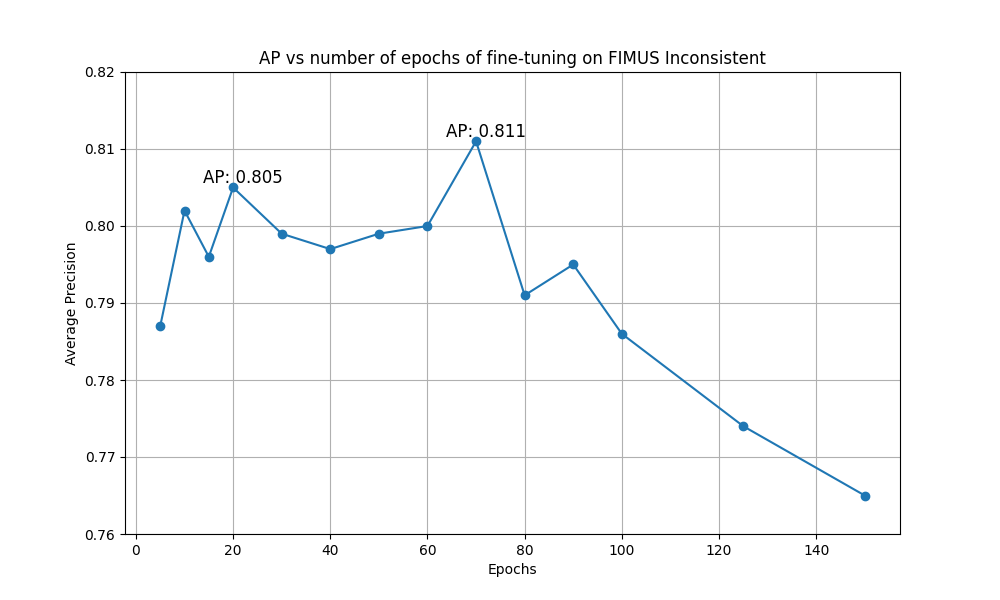
\includegraphics[width=\textwidth]{Images/Analytics/plot_AP_coco.png}
    \caption{COCO APs Over Number of Epochs Fine Tuned on Inconsistent.}
    \label{fig:plot_AP_COCO}
\end{figure}

The following table (\ref{tab:APs_models_COCO}) displays how well the models performed on the Consistent dataset. 

\begin{table}[H]
    \centering
    \renewcommand{\arraystretch}{1.5}
    \setlength{\tabcolsep}{1em}
    \begin{tabular}{|l|c|c|c|c|}
        \hline
        \rowcolor{gray!25}
        \textbf{Model} & \textbf{AP50} & \textbf{AP75} & \textbf{AP90} & \textbf{AP50-95} \\ \hline
        YOLOv9-m Not Fine-Tuned         & 0.957 & 0.908 & 0.768 & 0.865 \\ \hline
        YOLOv9-c Not Fine-Tuned         & 0.932 & 0.885 & 0.757 & 0.845 \\ \hline
        YOLOv9-e Not Fine-Tuned         & 0.972 & 0.949 & 0.912 & \textbf{0.945 }\\ \hline
        YOLOv9 CrowdHuman 5ep           & 0.968 & 0.916 & 0.707 & 0.834 \\ \hline
        YOLOv9 CrowdHuman 10ep          & 0.964 & 0.914 & 0.730 & 0.831 \\ \hline
        YOLOv9 Inconsistent 20ep        & 0.950 & 0.850 & 0.662 & 0.805 \\ \hline
        YOLOv9 Inconsistent 70ep        & 0.954 & 0.867 & 0.657 & 0.811 \\ \hline
        YOLOv9 PRW 5ep                  & 0.802 & 0.681 & 0.347 & 0.605 \\ \hline
        YOLOv9 PRW 10ep                 & 0.969 & 0.856 & 0.269 & 0.721 \\ \hline
        YOLOv9 Football 5ep             & 0.214 & 0.143 & 0.143 & 0.143 \\ \hline
        YOLOv9 Football 10ep            & 0.286 & 0.190 & 0.143 & 0.176 \\ \hline
        YOLOv3                          & 0.804 & 0.742 & 0.510 & 0.681 \\ \hline
        DETR-50                         & 0.776 & 0.711 & 0.369 & 0.624 \\ \hline
        DETR-101                        & 0.818 & 0.762 & 0.408 & 0.665 \\ \hline
\end{tabular}
\caption[COCO APs Comparison of Various Models on Consistent.]{COCO APs comparison of various models on Consistent (757 images).}
\label{tab:APs_models_COCO}
\end{table}

\phantomsection
\label{sec:table_discussion}
These are disappointing results, showing no improvement in the models from implementing the fine-tuning. The models that were not fine-tuned performed best on the Consistent dataset, showing how freezing the backbone and fine-tuning the head on inconsistent, highly relevant data was a destructive practice in this case and did not improve the model accuracies. 

Out of the fine-tuned models, the best performant one was the YOLOv9 model trained on the CrowdHuman dataset for 5 epochs. This is not unexpected: The dataset contains a lot of diversity and probably more instances of humans to learn from than the Inconsistent FIMUS dataset. The models that were fine-tuned on Inconsistent were trained for a tenfold more epochs to try to make up for this fact, but the accuracies failed to improve. These results indicate that rather than producing a sub-optimal specialized dataset for fine-tuning a model, the better option may be to use a larger and better dataset. 

Should the positioning of the bounding boxes be of less importance, we see that fine-tuning on the PRW dataset is still a better option than fine-tuning on our FIMUS Inconsistent dataset partition. This is revealed by the AP50 score of 0.969 after just 10 epochs, while training on FIMUS Inconsistent did not achieve similar results in it's 150 epochs of training. 

Further, we see that the models fine-tuned on the football player dataset were really bad-performing. They both completely missed the persons in the aquarium. This is likely largely due to the difference in scale, resulting in a fine-tuned model not able to predict the humans in the aquarium setting. A review of the labels indicate that the model had close to no inferences with a confidence score higher than 0.1, and the highest confidence at 0.425. An attempt was made to improve the scores by normalizing the detections, which resulted in the reported AP50-95 of 0.176 for the 10 epoch model, and 0.143 for the 5 epoch model. Prior to the confidence score adjustment, both models scored 0.0. 

The fixed confidence threshold was raised for the DETR models since they report vastly higher confidence scores than many other model architectures. Therefore, the confidence scores were fixed at 0.99. A comparison of the inference latencies of the models were not conducted, as the YOLO model is still clearly the better option. For Table \ref{tab:APs_models_both}, the confidence threshold was varied similar to every other model.

Another surprising result from Table \ref{tab:APs_models_COCO} is the YOLOv9-m performance relative to the larger weights of c and e! These letters correspond to different pre-trained weights, with various number of parameters. The converted version\footnote{There's also converted vs not converted models. The reparameterization functionality to convert a model consists of trimming layers meant to speed up and augment model training, which is not needed for running model inference. The converted models achieve the same results but with lower inference latency, smaller size. They should not, however, be used for fine-tuning.} of YOLOv9-e weight file has a size of 117.2MB, YOLOv9-c and -e fills only respectively 51.4MB and 40.7MB of space.

\paragraph{Vary-Both AP}
Figure \ref{fig:plot_AP_both} displays how the AP of the models varied with number of epochs. Equally to the COCO AP, the best model was the standard YOLOv9-e. We recall the Vary-Both AP references to the AP score achieved when evaluating models with a varying IoU threshold of 10 values from 0.50-0.95 \textit{and} confidence threshold from 0.10 to 0.90 in 20 steps.   

\begin{figure}[H]
    \centering
    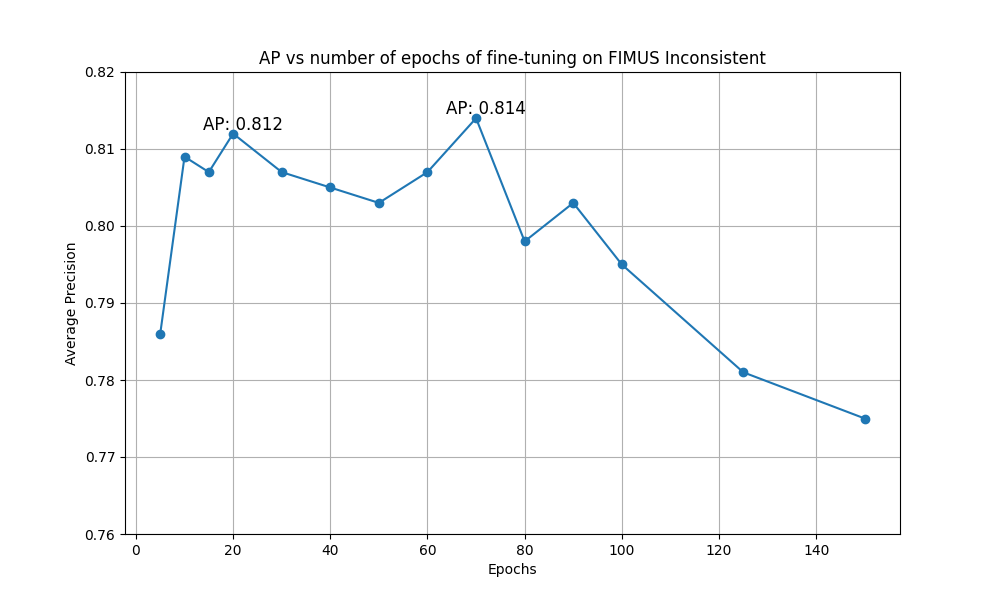
\includegraphics[width=\textwidth]{Images/Analytics/plot_AP_both.png}
    \caption{Vary-Both APs Over Number of Epochs Fine Tuned on Inconsistent.}
    \label{fig:plot_AP_both}
\end{figure}

The following table (\ref{tab:APs_models_both}) displays how well the models performed on the Consistent dataset. Similarily to the results in Table \ref{tab:APs_models_COCO}, the YOLOv9-e was the most accurate, achieving an AP50-95 of 0.913. 

\begin{table}[H]
    \centering
    \renewcommand{\arraystretch}{1.5}
    \setlength{\tabcolsep}{1em}
    \begin{tabular}{|l|c|c|c|c|}
        \hline
        \rowcolor{gray!25}
        \textbf{Model} & \textbf{AP50} & \textbf{AP75} & \textbf{AP90} & \textbf{mAP50-95} \\ \hline
        YOLOv9-m Not Fine-Tuned          & 0.895 & 0.855 & 0.746 & 0.821 \\ \hline
        YOLOv9-c Not Fine-Tuned          & 0.881 & 0.842 & 0.740 & 0.810 \\ \hline
        YOLOv9-e Not Fine-Tuned          & 0.942 & 0.918 & 0.876 & \textbf{0.913} \\ \hline
        YOLOv9 on Inconsistent for 20ep  & 0.948 & 0.854 & 0.680 & 0.812 \\ \hline
        YOLOv9 on Inconsistent for 70ep  & 0.948 & 0.867 & 0.674 & 0.814 \\ \hline
        YOLOv9 on PRW for 5ep            & 0.808 & 0.706 & 0.427 & 0.633 \\ \hline
        YOLOv9 on PRW for 10ep           & 0.924 & 0.792 & 0.252 & 0.677 \\ \hline
        YOLOv9 on CrowdHuman for 5ep     & 0.908 & 0.863 & 0.688 & 0.788 \\ \hline
        YOLOv9 on CrowdHuman for 10ep    & 0.944 & 0.902 & 0.740 & 0.822 \\ \hline
        YOLOv9 on Football for 5ep       & 0.221 & 0.177 & 0.175 & 0.179 \\ \hline
        YOLOv9 on Football for 10ep      & 0.514 & 0.457 & 0.443 & 0.452 \\ \hline
        YOLOv3                           & 0.780 & 0.728 & 0.528 & 0.672 \\ \hline
        DETR ResNet50                    & 0.414 & 0.355 & 0.164 & 0.315 \\ \hline
        DETR ResNet101                   & 0.594 & 0.526 & 0.245 & 0.460 \\ \hline
    \end{tabular}
    \caption{APs Comparison of Various Models on Consistent (757 images), Varying Both Thresholds.}
    \label{tab:APs_models_both}
\end{table}

Results are similar to those in Table \ref{tab:APs_models_COCO}. See \ref{sec:table_discussion} for a brief presentation of the results. Note that for this evaluation, the DETR models were also varied from 0.1 to 0.90 in confidence thresholds, resulting in much worse average precisions.

\paragraph{DETR Fixed Confidence Thresholds' Effects on Average Precision}
The poor performances of the DETR models motivated the an investigation of the labels. The DETR models infer with much higher confidences, making the fixed threshold at 0.5 way too low to score well on the COCO metric. An assessment was made thus made to find the optimal confidence level for the model. This was found at 0.991, nearly doubling the AP score from 0.315 to 0.625 for the DETR with a ResNet50 backbone, and improving the score from 0.460 to 0.668 for the model with the more complex ResNet101 backbone.

\begin{table}[H]
    \centering
    \renewcommand{\arraystretch}{1.5}
    \setlength{\tabcolsep}{1em}
    \begin{tabular}{|l|c|c|c|c|}
        \hline
        \rowcolor{gray!25}
        \textbf{Model} & \textbf{AP50} & \textbf{AP75} & \textbf{AP90} & \textbf{mAP50-95} \\ \hline
        DETR ResNet50 Conf  0.50             & 0.414 & 0.355 & 0.164 & 0.315 \\ \hline
        DETR ResNet50 Conf  0.95             & 0.755 & 0.660 & 0.326 & 0.585 \\ \hline
        DETR ResNet50 Conf  0.99             & 0.776 & 0.711 & 0.369 & 0.624 \\ \hline
        DETR ResNet50 Conf  0.991            & 0.773 & 0.713 & 0.373 & 0.625 \\ \hline
        DETR ResNet101 Conf 0.50             & 0.594 & 0.526 & 0.245 & 0.460 \\ \hline
        DETR ResNet101 Conf 0.95             & 0.795 & 0.719 & 0.353 & 0.627 \\ \hline
        DETR ResNet101 Conf 0.99             & 0.818 & 0.762 & 0.408 & 0.665 \\ \hline
        DETR ResNet101 Conf 0.991            & 0.818 & 0.767 & 0.419 & 0.668 \\ \hline
    \end{tabular}
    \caption{APs for DETR When Fixing the Confidence Threshold at Various Values (757 images).}
    \label{tab:DETR_conf}
\end{table}

The results presented in Table \ref{tab:DETR_conf} are in accordance with the results of \citeauthor{carion2020endtoend}. They claim it is performing well on panoptic segmentation, a task where pixel-level detail is important. This is the reason to the confidence values are high for the task of object detection. For the experiments in Table \ref{tab:APs_models_COCO}, a threshold of 0.99 was used instead of 0.991, because experimentally finding the optimal confidence threshold post-inference on a test-set is likely overfitted to the testing data and not so easy to optimize for in a practical setting.

The results of this section are put into a broader context in the Discussion section, see \ref{sec:broader_context}.

\subsection{Data Visualization}
\label{sec:data_visualization}
The data may be visualized a multiple of ways. The explored methods in this thesis are by creating heat maps and bar charts to visualize the data. 

\subsubsection{Heatmaps}
\label{sec:results_heatmaps}
As mentioned in Section \ref{sec:heatmaps}, heatmaps are a powerful visualization tool that can provide insights into visitor behavior patterns and engagement levels within a museum or aquarium setting. Heatmaps for the month of may are illustrated in \ref{fig:heatmap_final}. These heatmap generation code for the two heatmaps are identical, apart from one variable: the position where detections are mapped to. In \ref{fig:heatmap_final}a and b, the detections are mapped to the respectively the middle and the bottom center of the detection bounding box. This single modification has the largest difference on the edges of occlusions, such as (for the images in Figure \ref{fig:heatmap_final}) the railing of the fish tank in the center.

\begin{figure}[H]
    \centering
    \begin{subfigure}{0.475\textwidth}
        \centering
        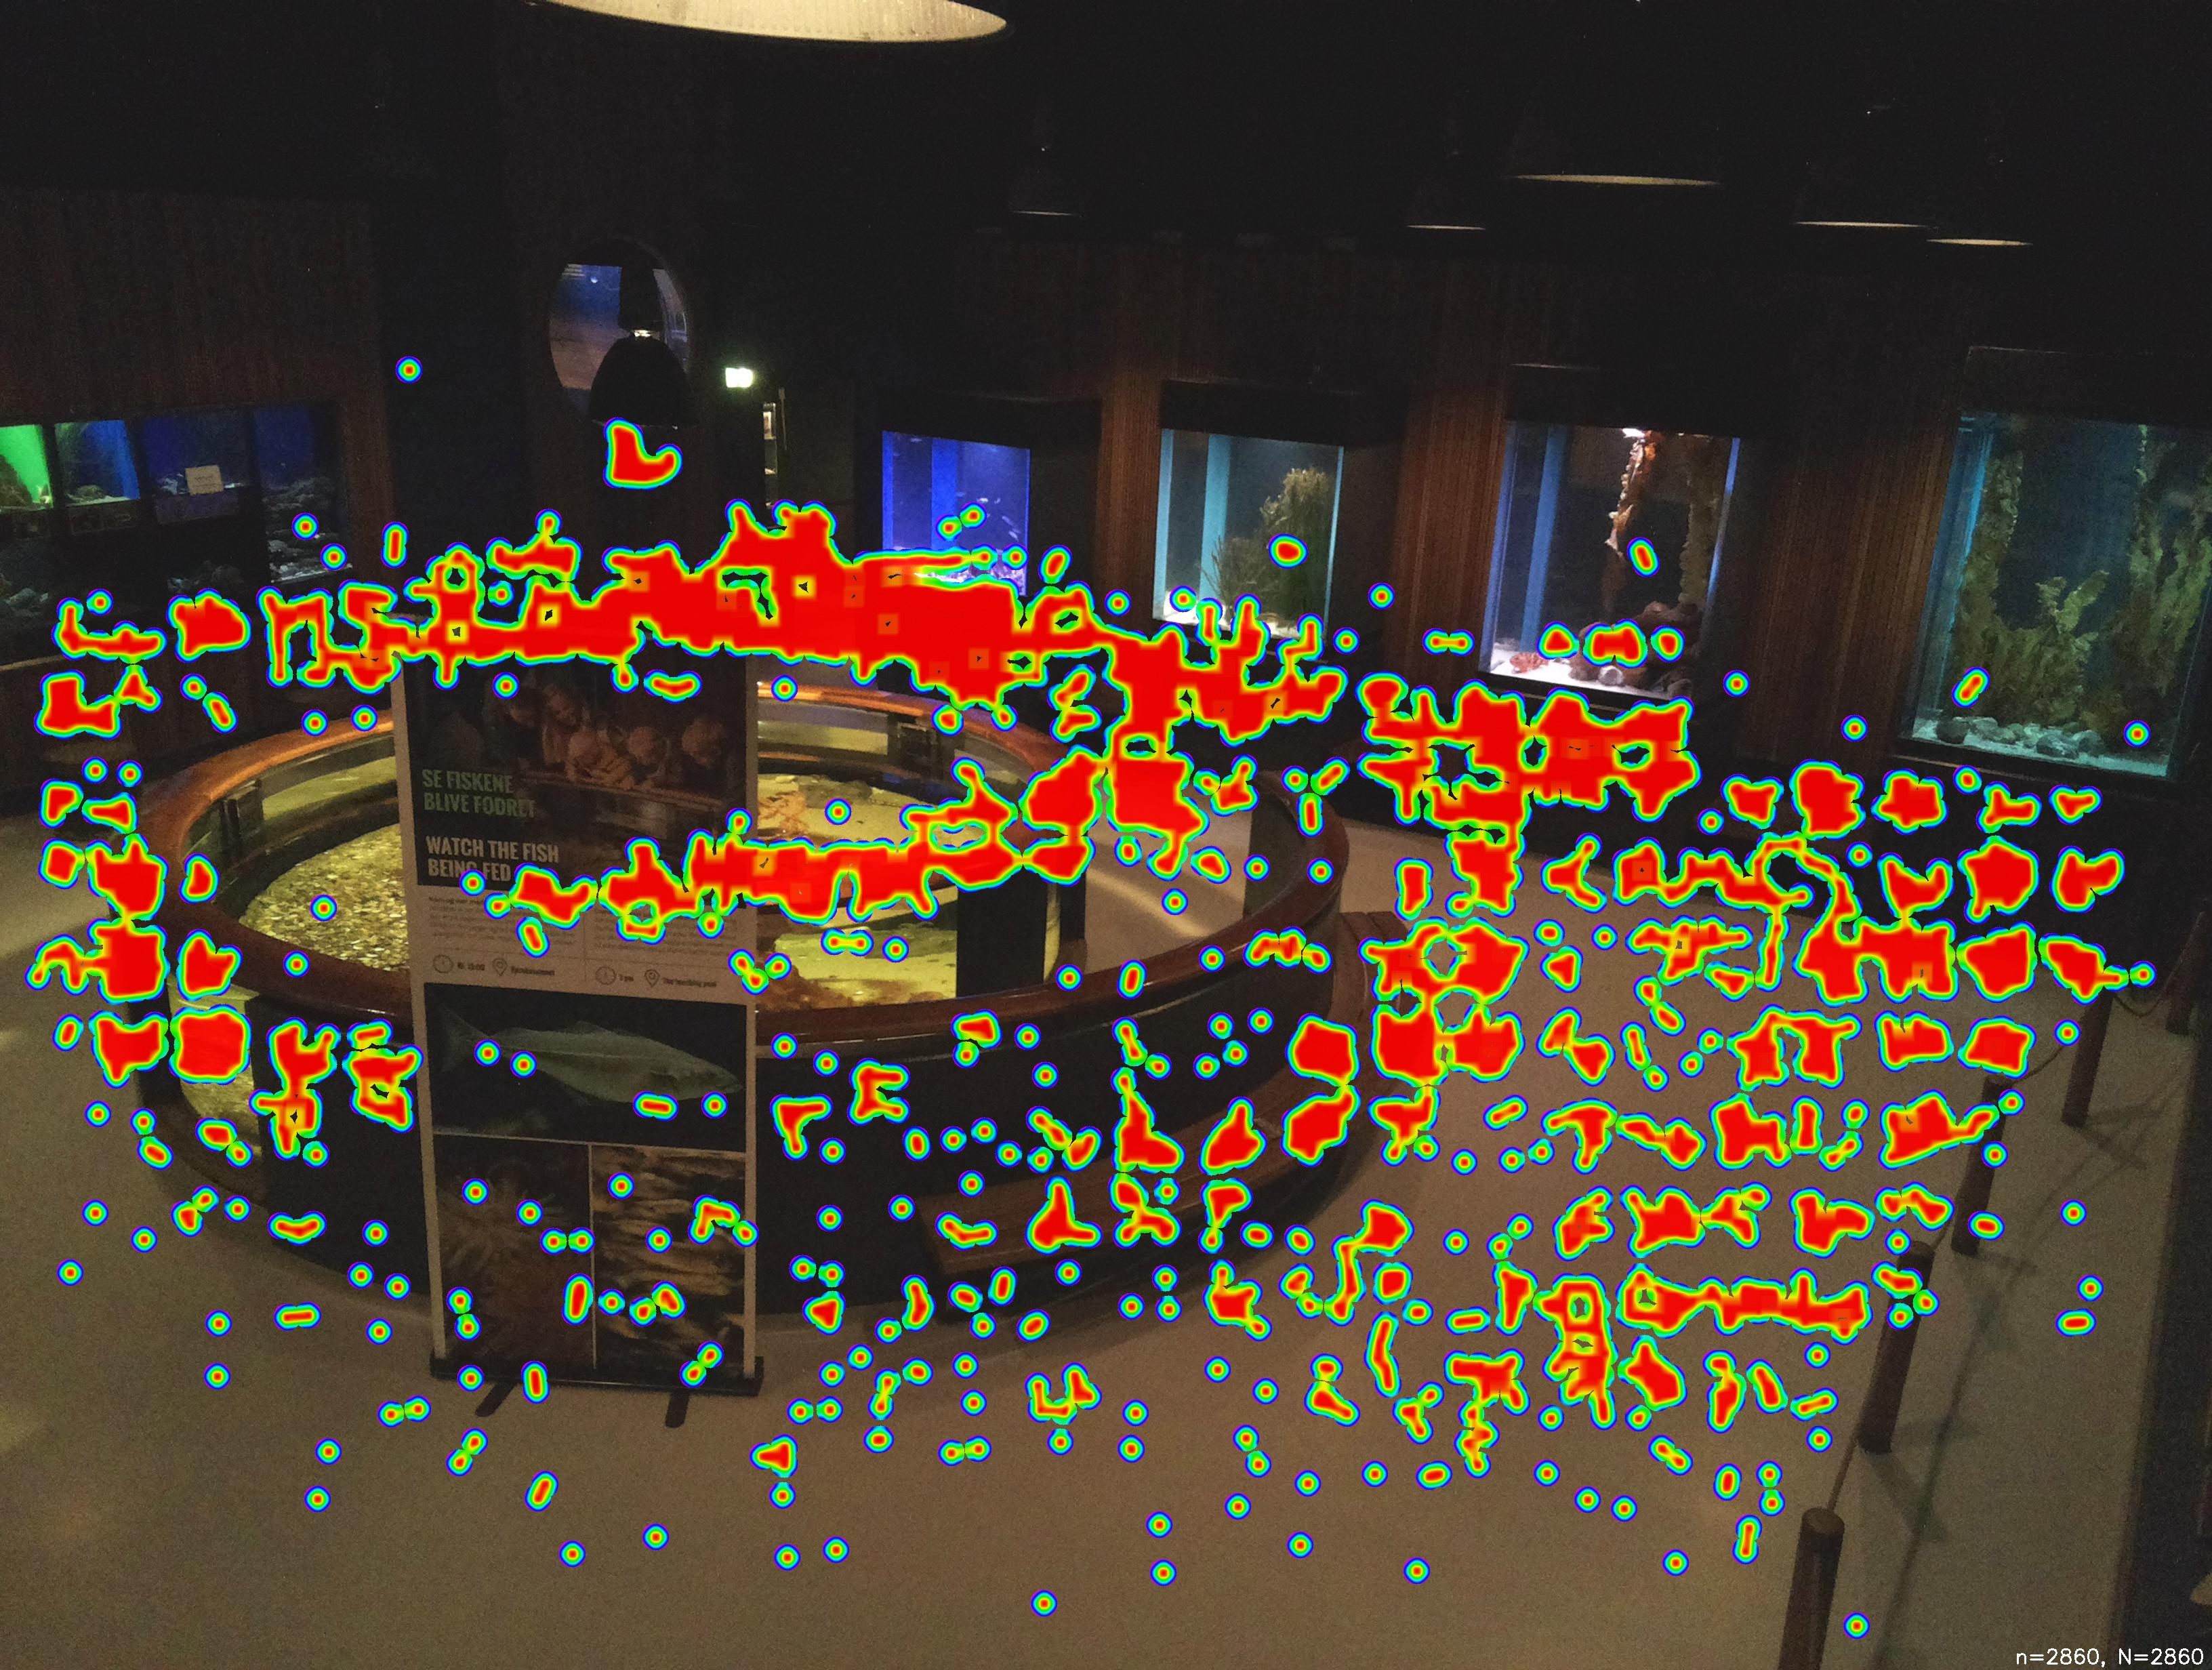
\includegraphics[width=\textwidth]{Images/Analytics/heatmap_supervision.jpg}
        \caption{Final Heatmap: Supervision, sampled from the \textit{middle} of detections}
    \end{subfigure}
    \hfill
    \begin{subfigure}{0.475\textwidth}
        \centering
        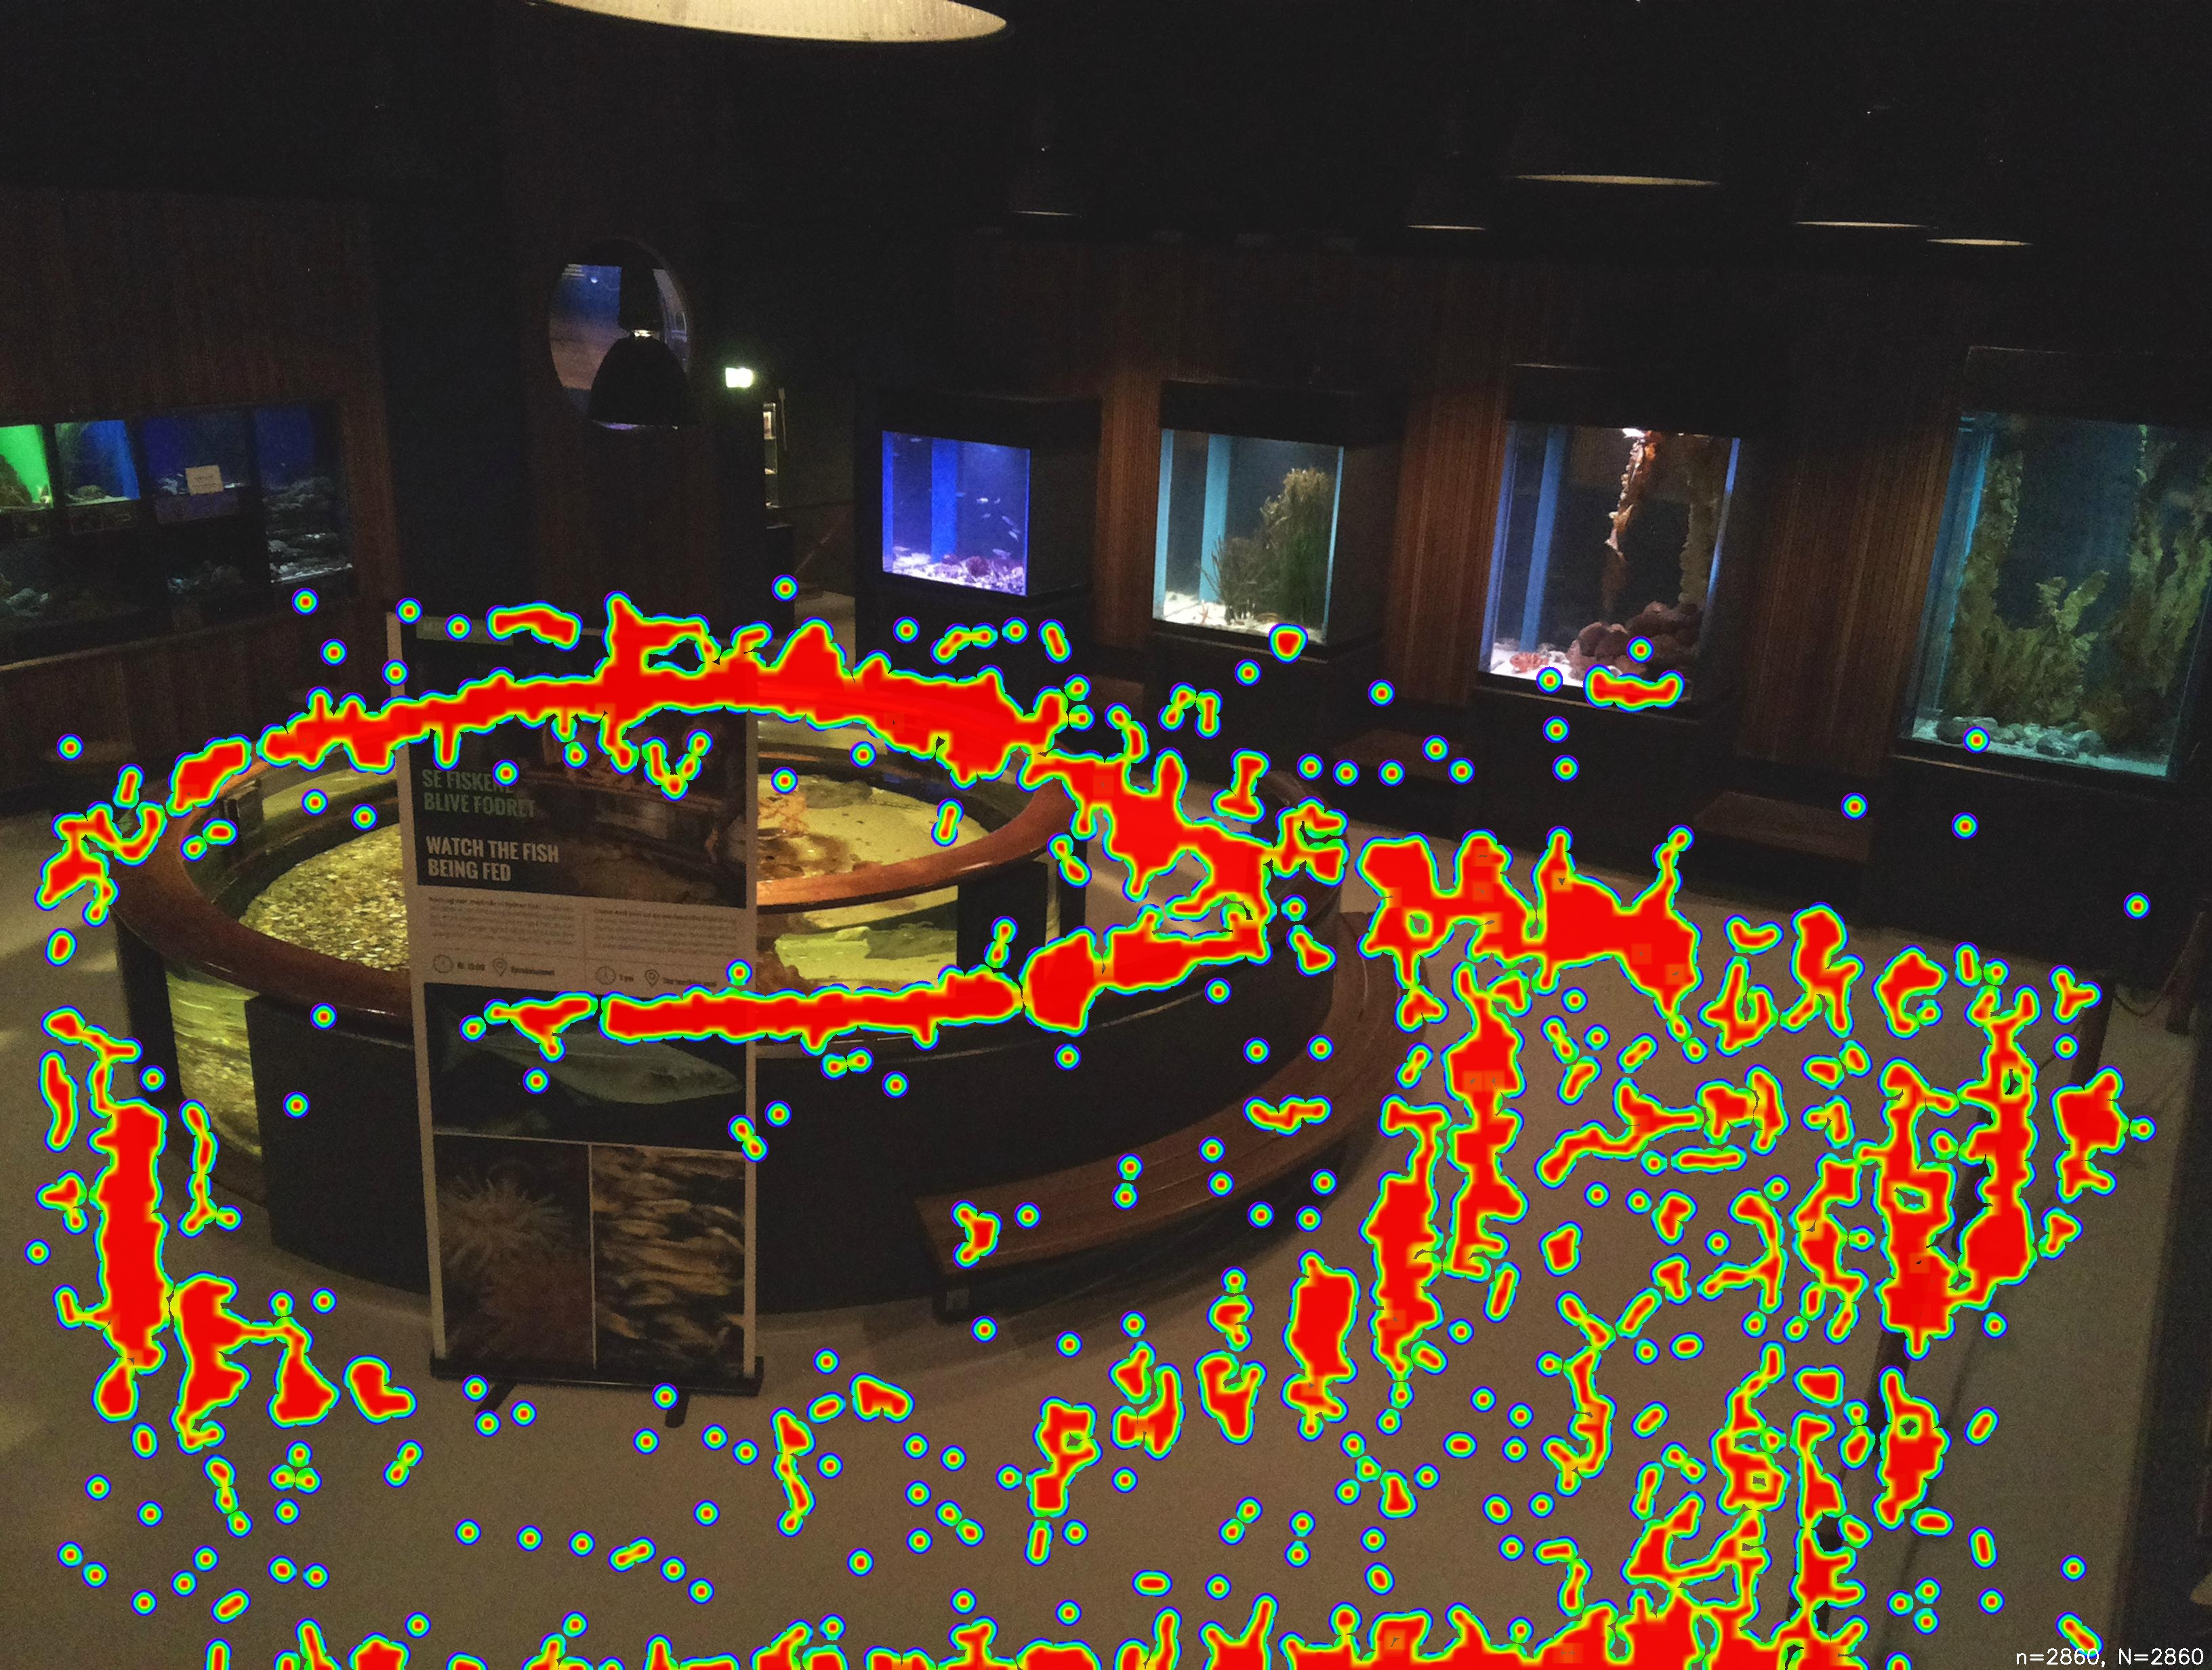
\includegraphics[width=1\textwidth]{Images/Analytics/heatmap_bottom_center.jpg}
        \caption{Final Heatmap: Supervision, sampled from the \textit{bottom} of detections}
    \end{subfigure}
    \caption{Final Heatmaps}
    \label{fig:heatmap_final}
\end{figure}

There's another, more important takeaway from the small modification. While seemingly similar, the heatmap sampling detections from the middle of the bounding boxes (\ref{fig:heatmap_final}a) reveal a weakness in our detector which is invisible in the other heatmap: the lamp is sometimes classified as a person. On the other hand, the other heatmap (\ref{fig:heatmap_final}b) reveal another weakness. The seaweed in the second fish tank from the right is sometimes also classified as a person.   

Apart from revealing weaknesses from the detector models\footnote{These weaknesses in our detector models could be revealed by looking at the annotated images. However, looking at the annotated images is not possible for a on-device processing image-deleting device. In this case, one would need to display/plot the detections onto a base-layer image (heat map), or make use of obfuscation discussed in Section \ref{sec:obfuscation} to illustrate and reveal model weaknesses.}, these heatmaps may provide valuable insights with regards to which areas of the facility are being used the most. There may be difficulties, however, in correctly inferring what are the reasons for the variations. For periods less than a day, these variations are likely due to randomness. The more interesting numbers in this context would be to see the total number of visitors throughout the day, which is better visualized in the bar charts in Section \ref{sec:peak_hours}. Two heatmaps for separate days are illustrated in Figure \ref{fig:heatmap_daily}.

\begin{figure}[H]
    \centering
    \begin{subfigure}{0.475\textwidth}
        \centering
        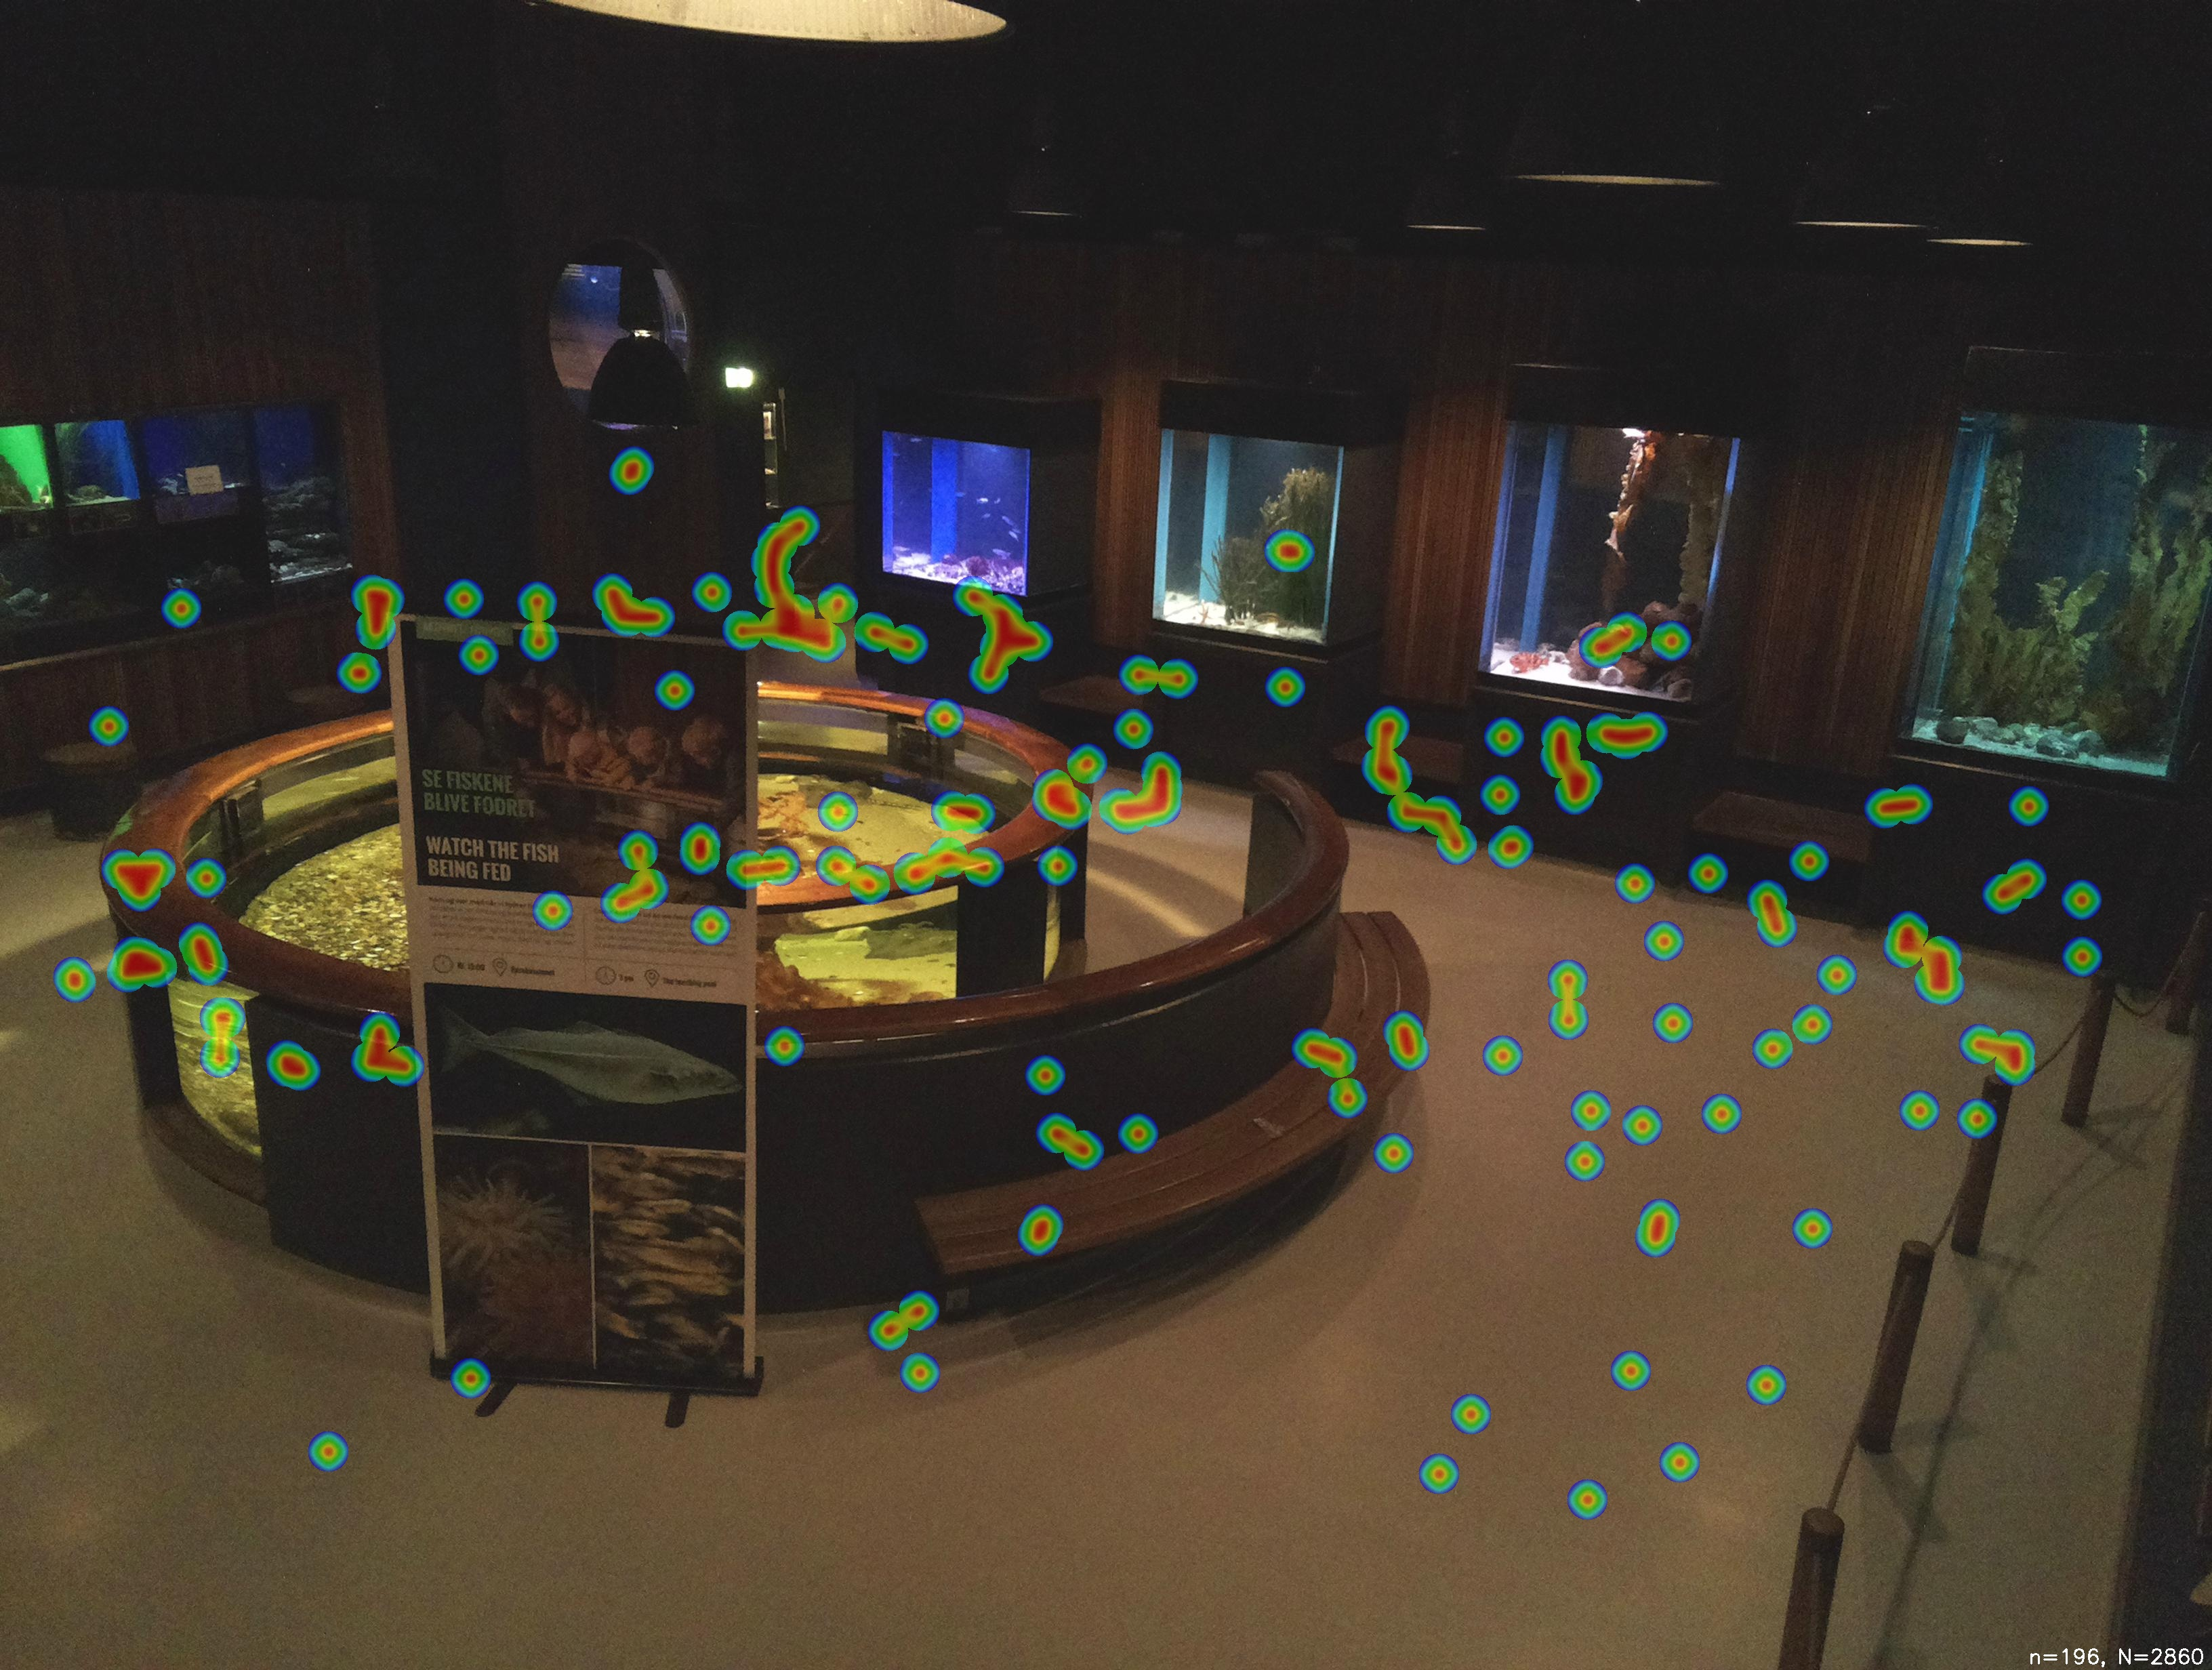
\includegraphics[width=\textwidth]{Images/Analytics/heatmap_day_08052024.jpg}
        \caption{Heatmap Wednesday 8th of May, 2024}
    \end{subfigure}
    \hfill
    \begin{subfigure}{0.475\textwidth}
        \centering
        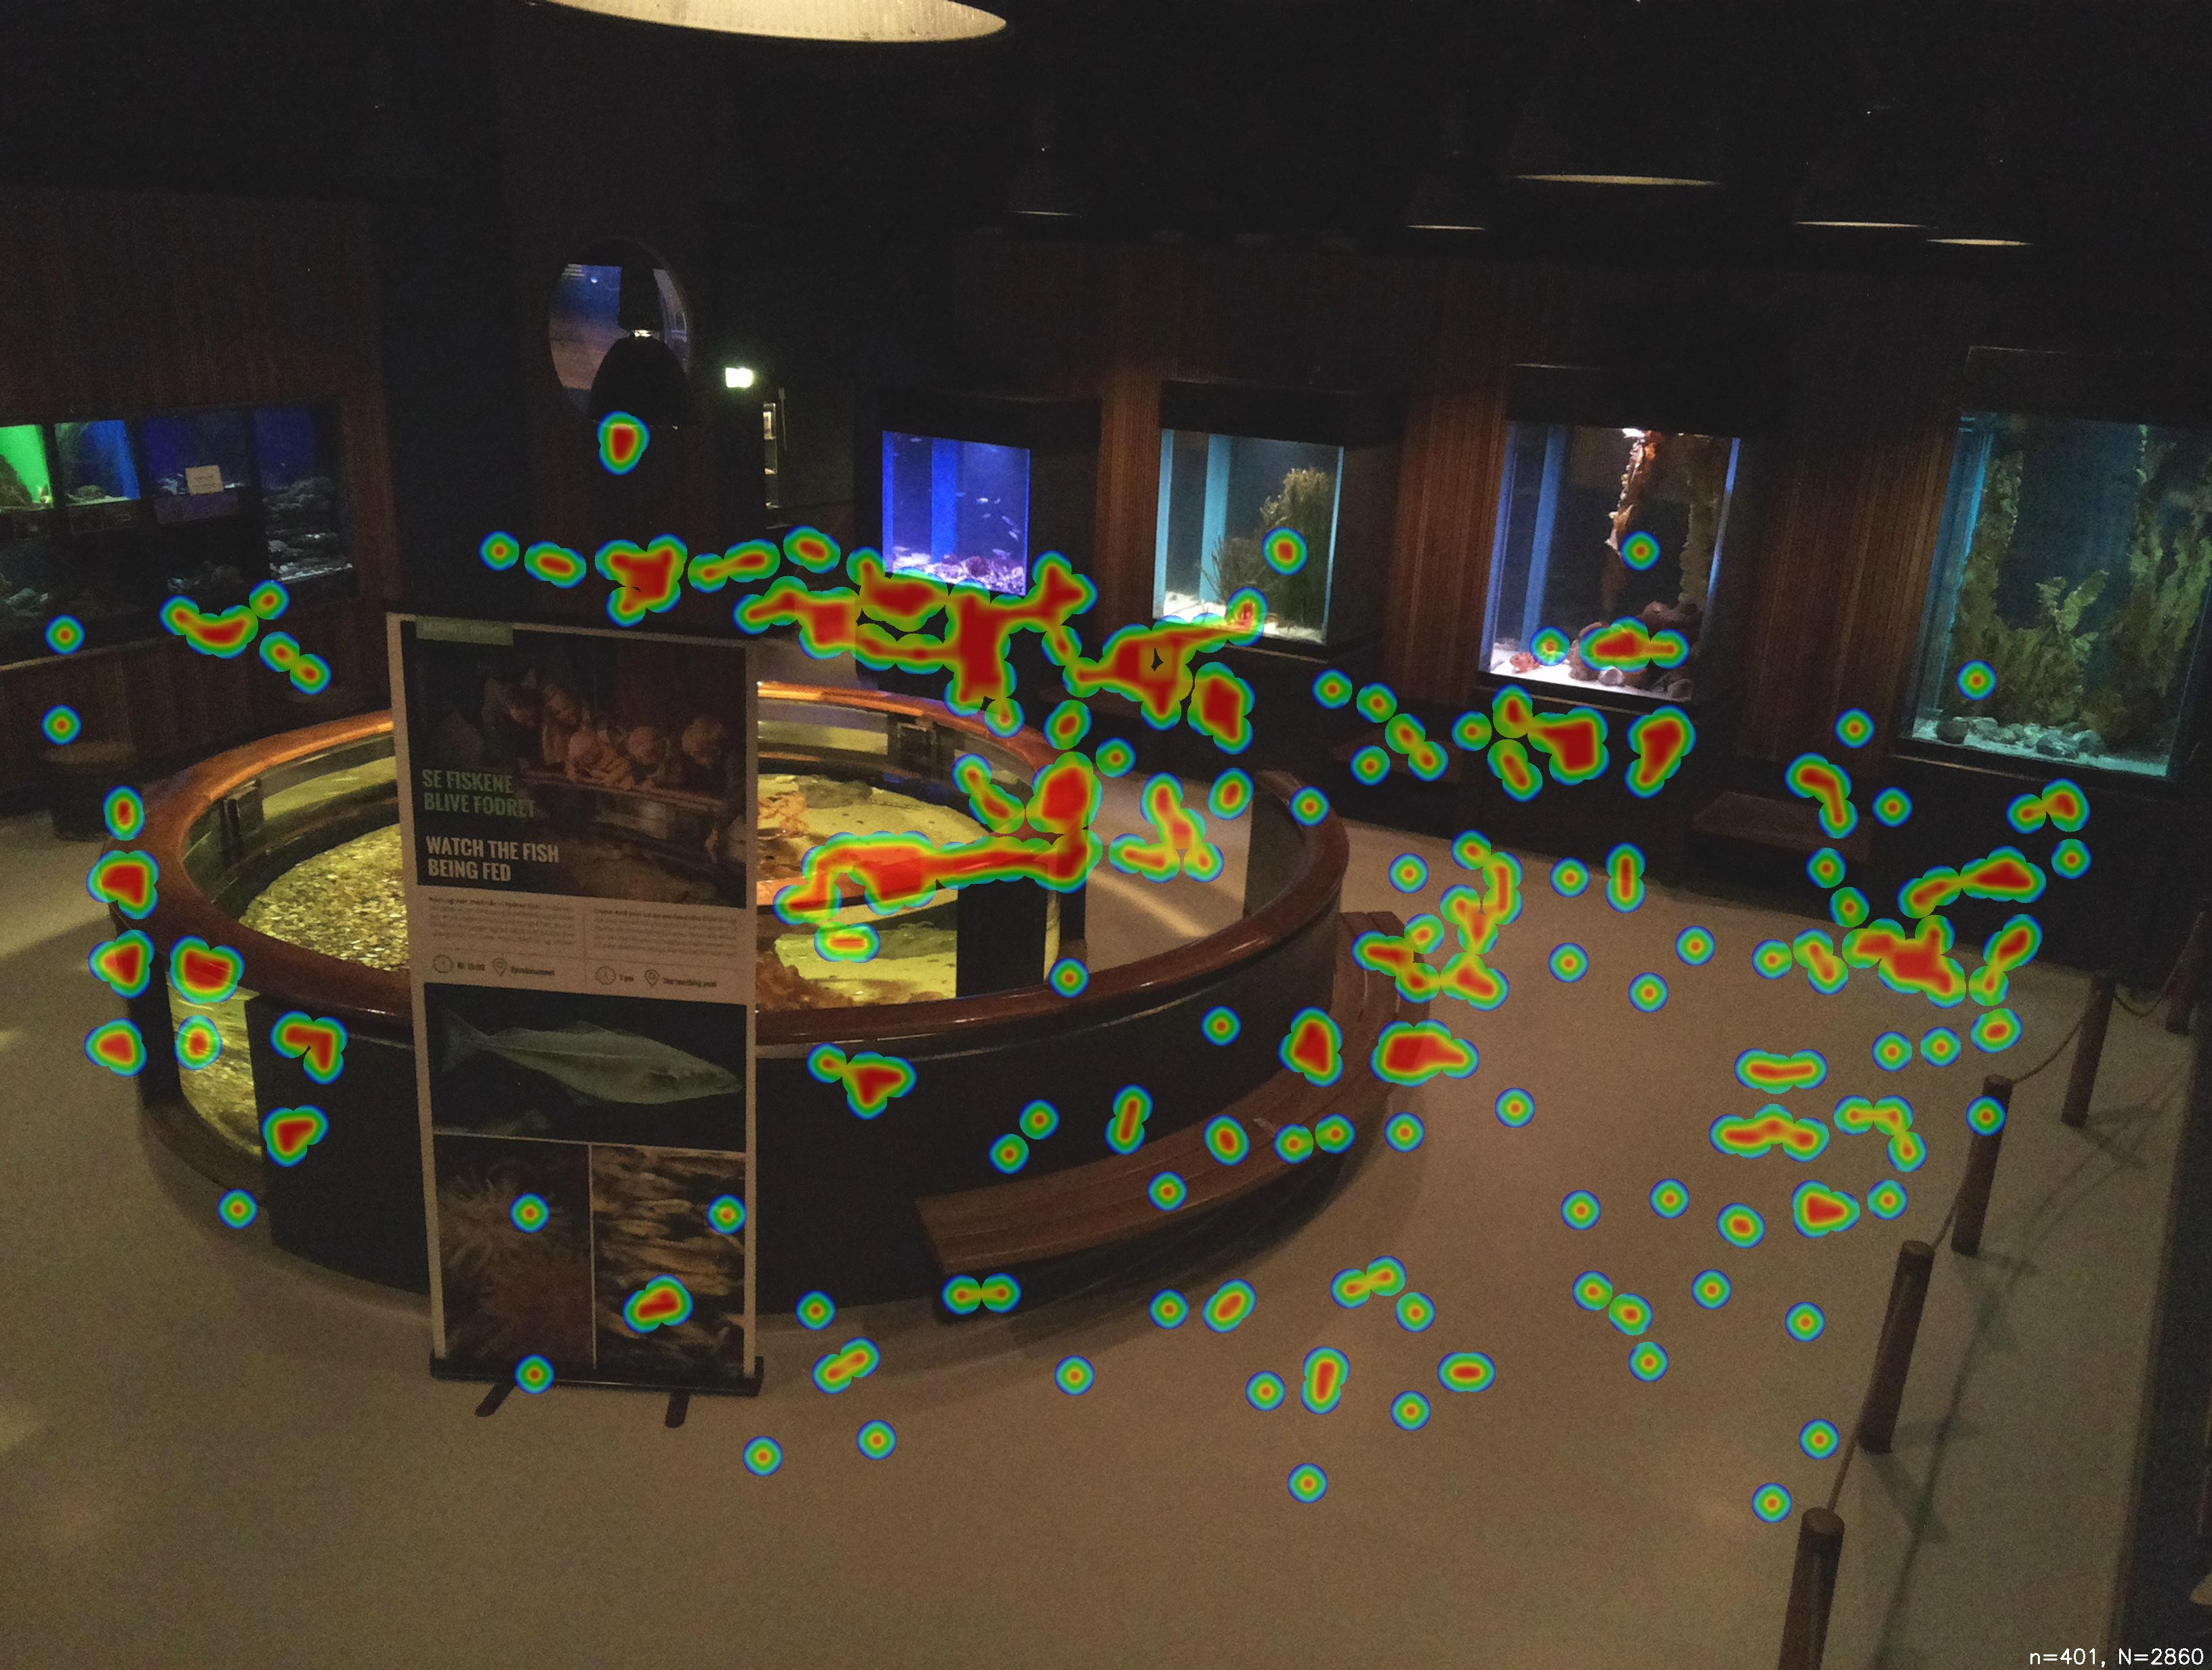
\includegraphics[width=1\textwidth]{Images/Analytics/heatmap_day_11052024.jpg}
        \caption{Heatmap Saturday 11th of May, 2024}
    \end{subfigure}
    \caption{Daily Heatmap}
    \label{fig:heatmap_daily}
\end{figure}

Heat maps may also visualize the hours throughout a day, accumulating all data for a specific time period each day to see if the visitor engagement changes based on the time. This is one example of introducing a variable, namely the time of day, to filter the detections. For an area where other variables such as the temperature, the noise level or the weather is also known, this could be used instead to filter the detections and illustrate how visitor engagement changes based on these factors. This usage would naturally, require some months-worth of data to be valid. For this project, only a months-worth of localization data has been stored to make the analysis. An illustration of heatmaps where the time of day has been used to determine which detections are presented in the heatmaps are displayed in Figure \ref{fig:heatmap_time}.

\begin{figure}[H]
    \centering
    \begin{subfigure}{0.475\textwidth}
        \centering
        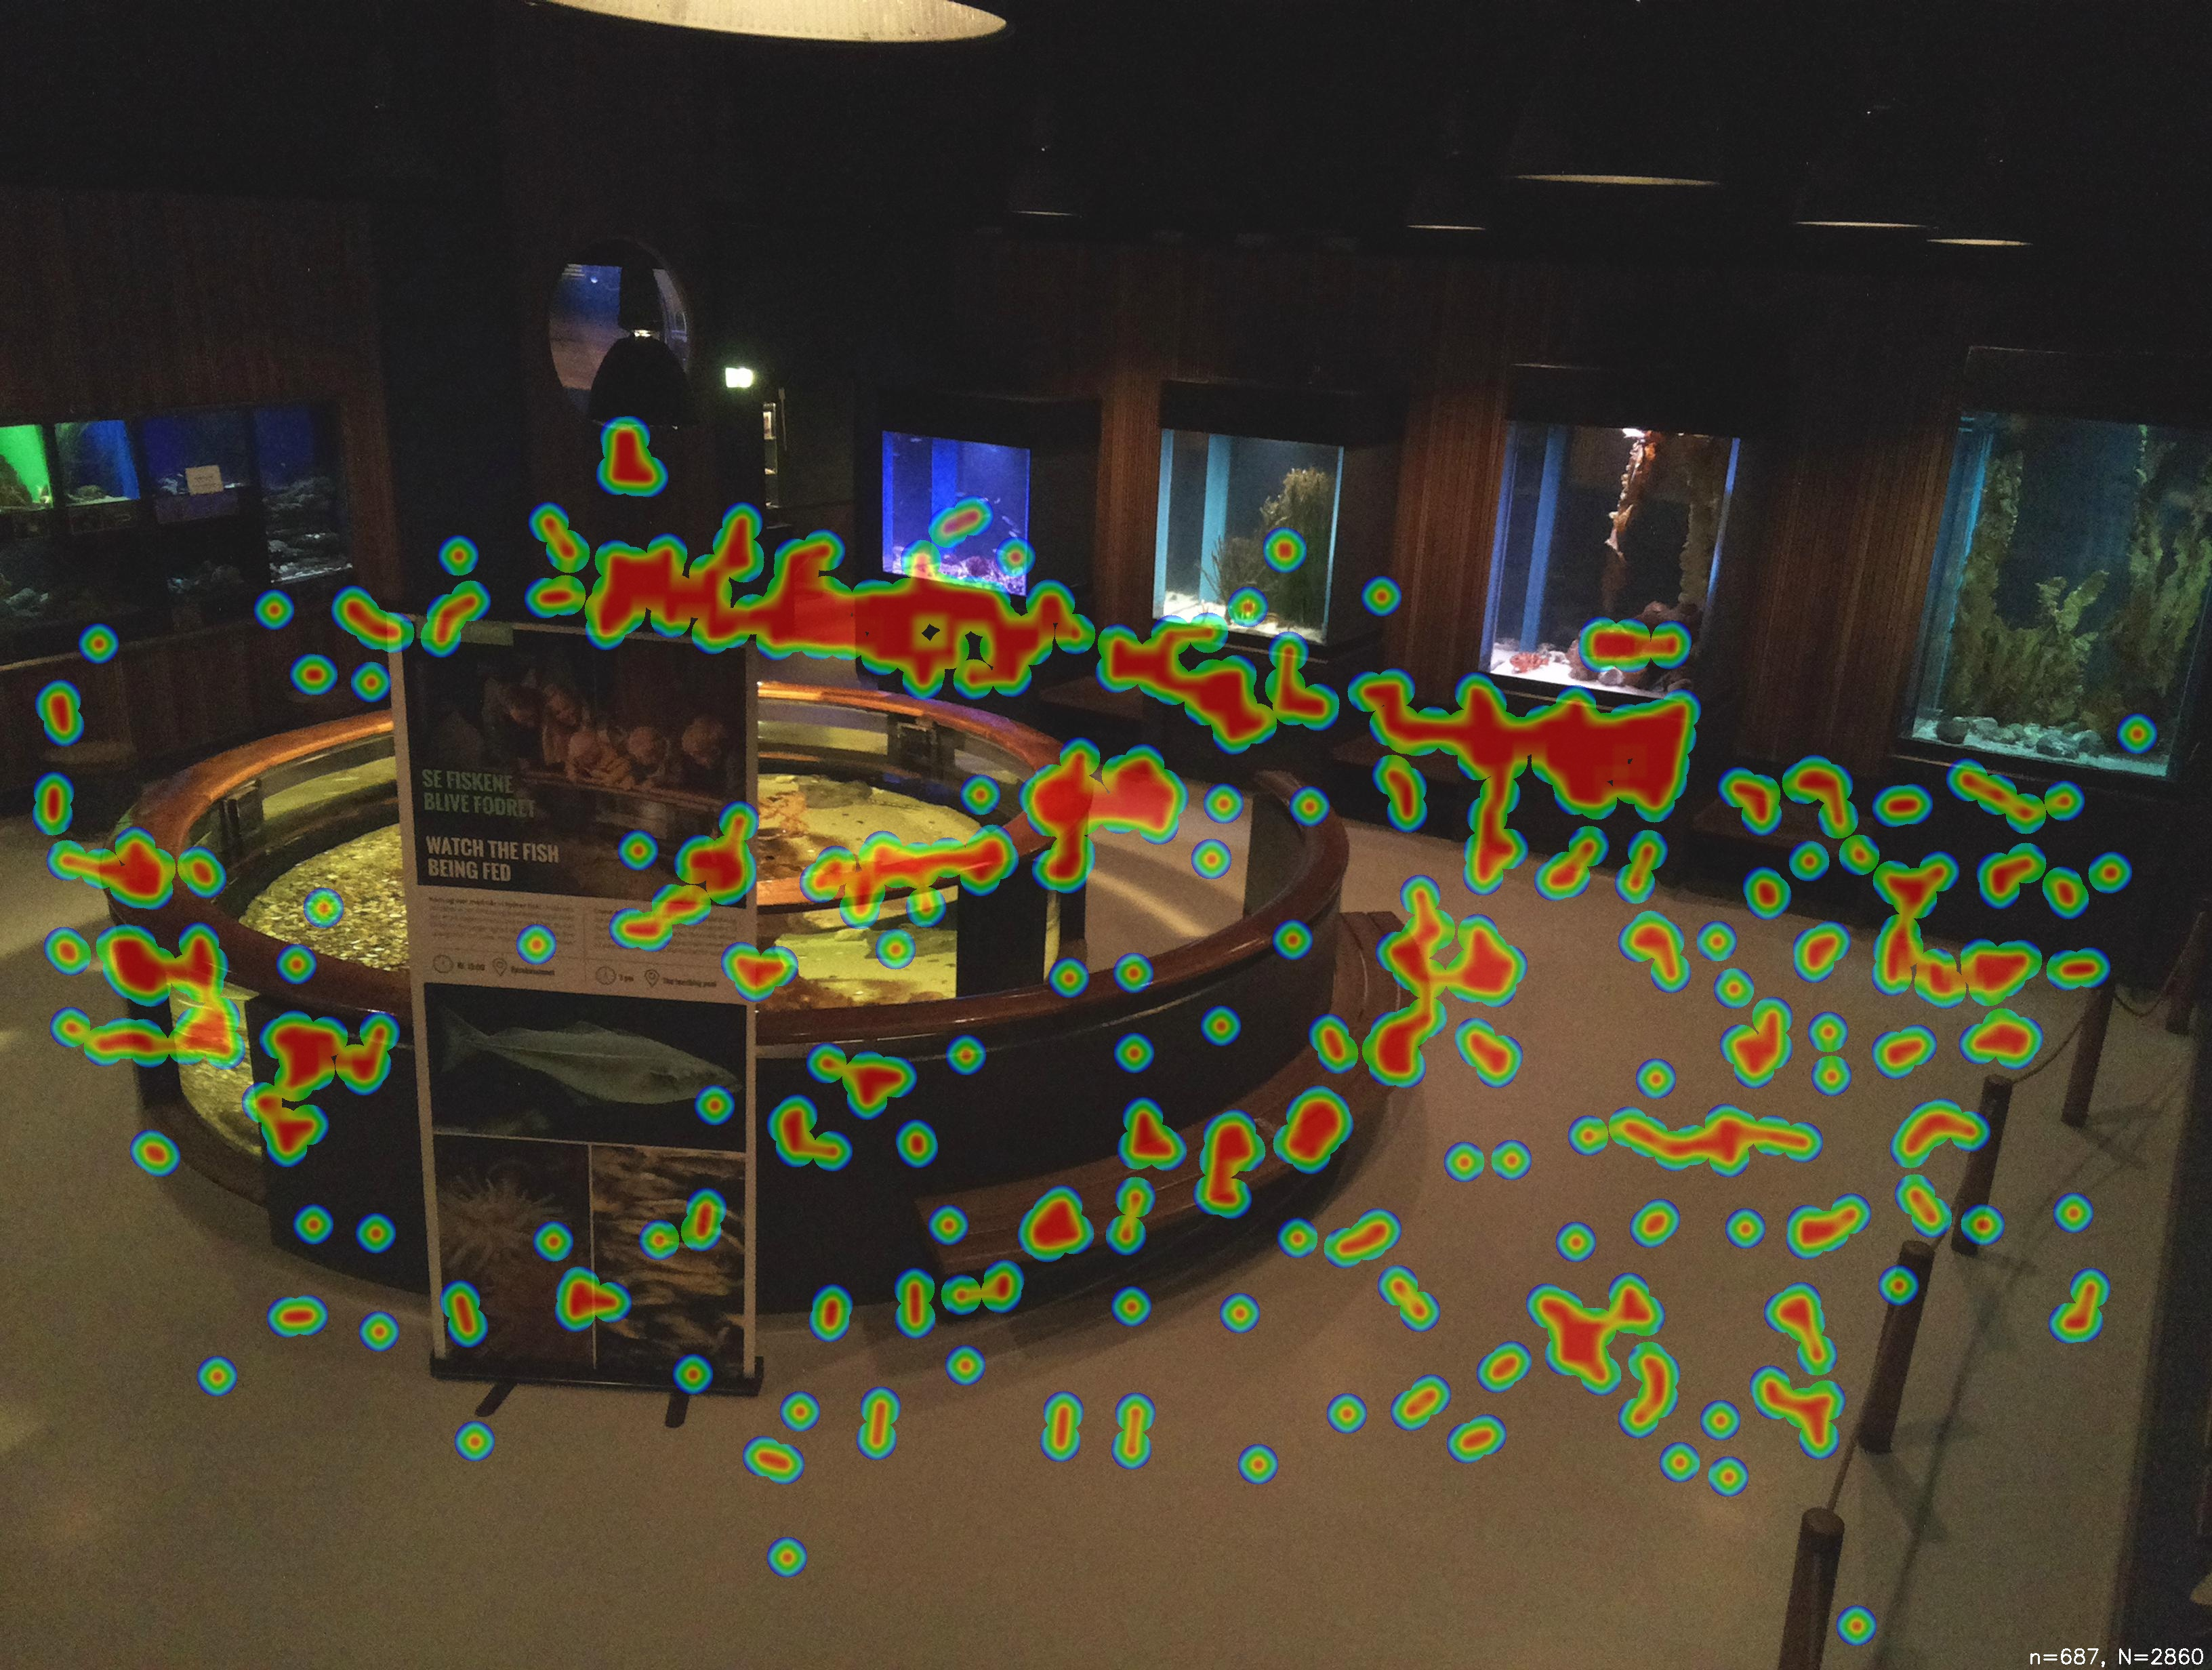
\includegraphics[width=\textwidth]{Images/Analytics/heatmap_time_1300_1400.jpg}
        \caption{Heatmap 13:00-14:00}
    \end{subfigure}
    \hfill
    \begin{subfigure}{0.475\textwidth}
        \centering
        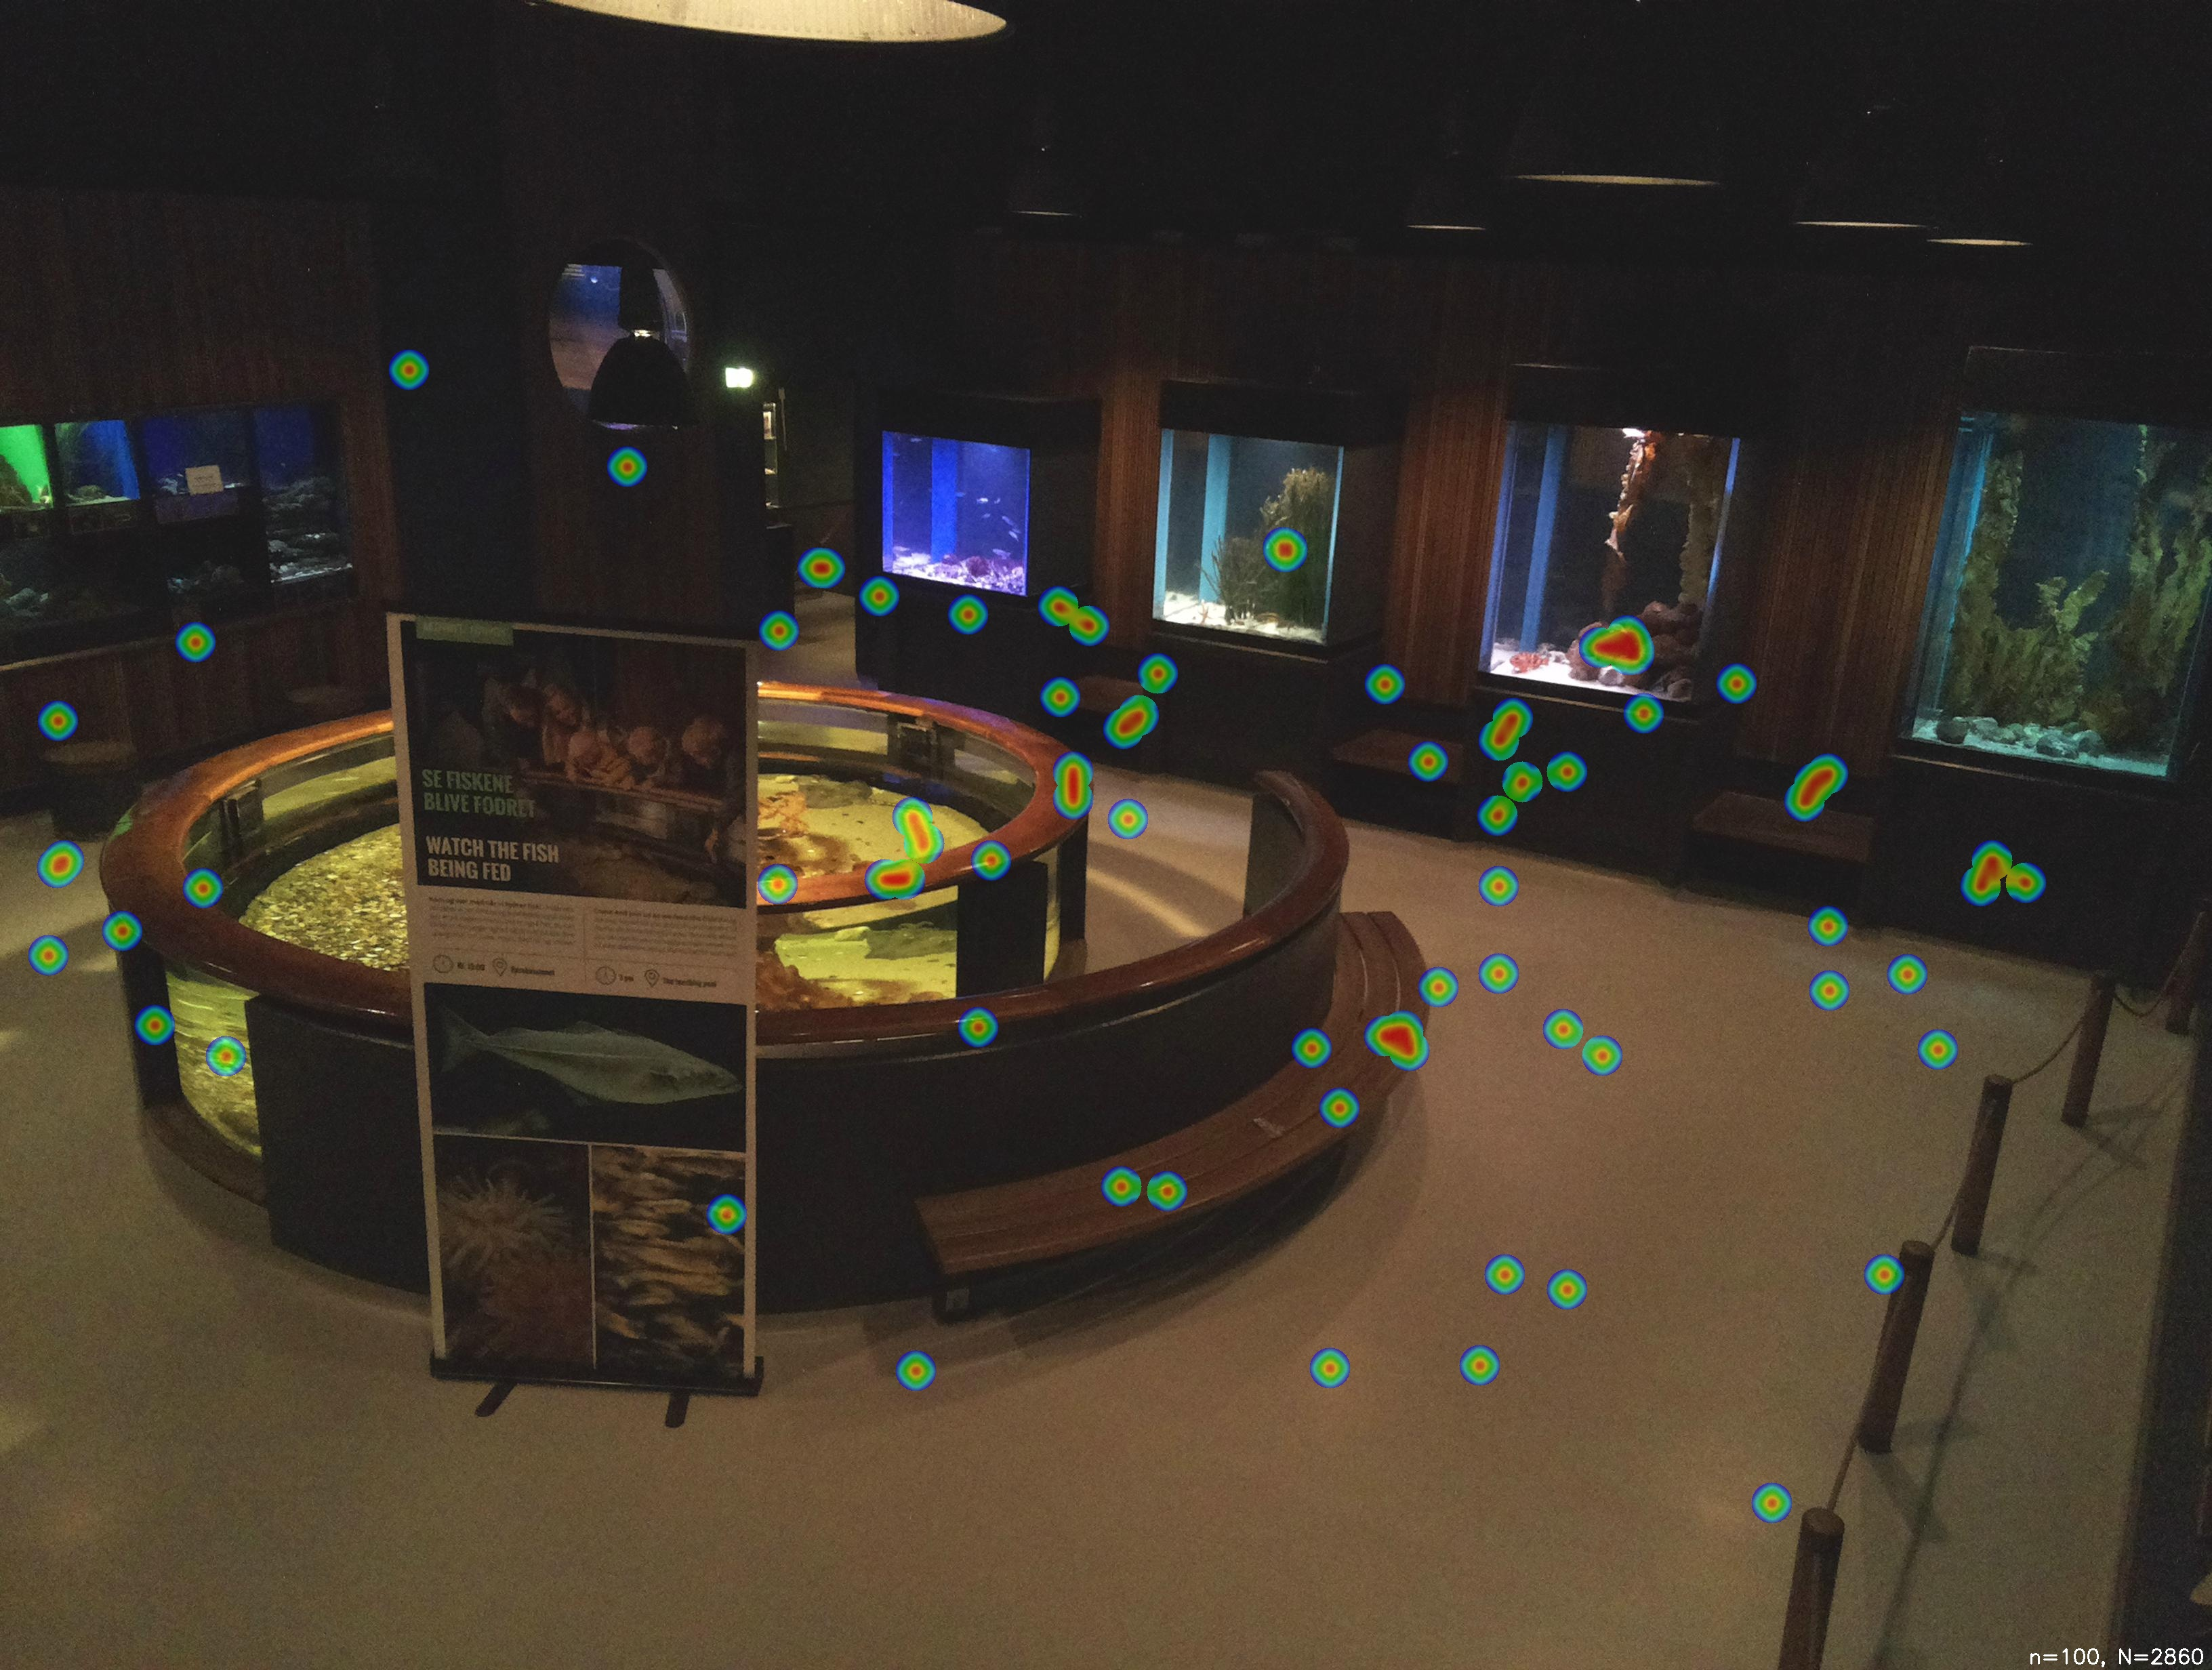
\includegraphics[width=1\textwidth]{Images/Analytics/heatmap_time_1600_1700.jpg}
        \caption{Heatmap 16:00-17:00}
    \end{subfigure}
    \caption{Hourly Heatmap}
    \label{fig:heatmap_time}
\end{figure}

The heatmaps in Figure \ref{fig:heatmap_time} reveal another use case for heatmaps. The relative difference between the two heatmaps is likely due to randomness, but with a larger number of detections one might be able to look for patterns. This could be that the heatmap for 13:00-14:00 could show a higher number of detections in front of the fish tanks, while the heatmap for 16:00-17:00 could show a higher number of detections on the benches. This could have easily been overlooked, had a manager of the museum only passed through the museum in the day and never in the evenings, resulting in him not thinking so many benches were neccessary. 


\subsubsection{Peak Hours}
\label{sec:peak_hours}
Another tool is to analyze the average number of detected persons per hour. This provides insights into room utilization during different times of the day.

\begin{figure}[H]
	\centering
	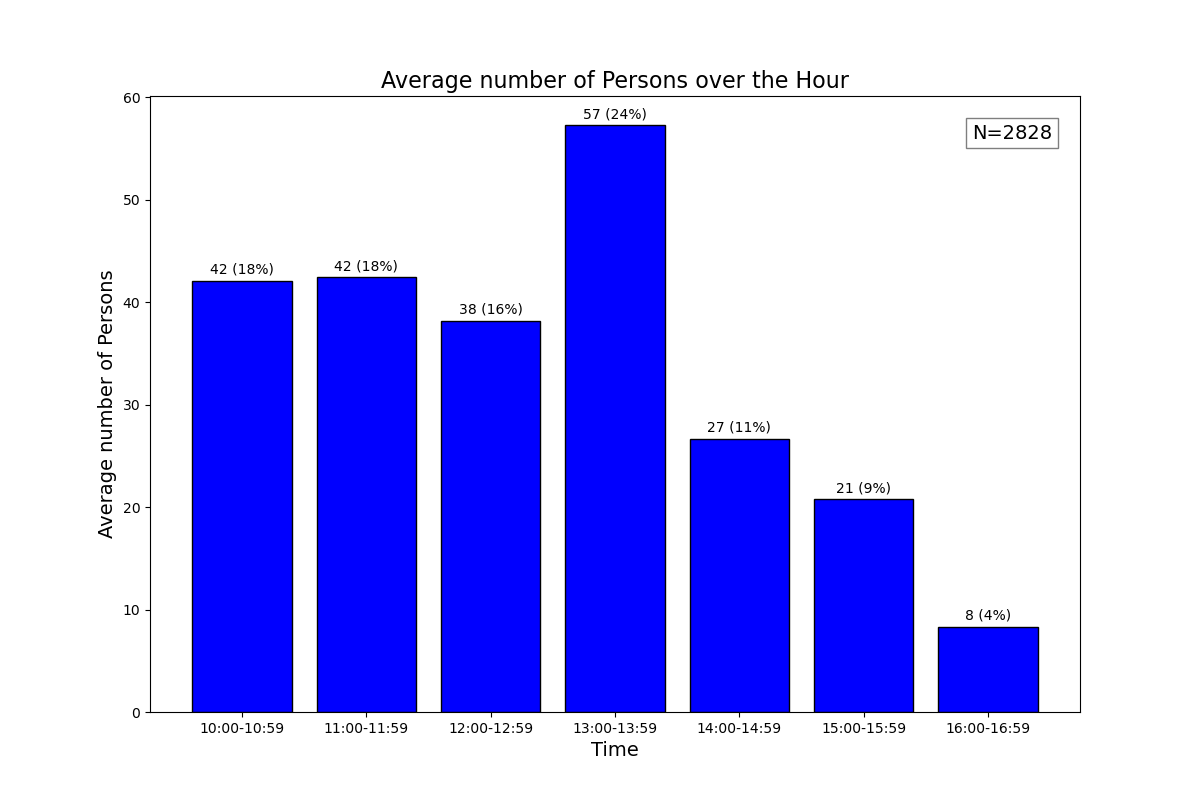
\includegraphics[width=1\textwidth]{Images/Analytics/peak_hours.png}
	\caption{Peak Hours Analysis}
    \label{fig:peak_hours}
\end{figure}

For instance, a lower number of detections during early opening hours, despite high visitor entry, could indicate that the room temperature is not yet optimal, affecting visitor comfort. This hypothesis could be tested by using the number of visitors as the dependent variable and adjust the room temperature to see the effects. In the absence of other confounding variables\footnote{Which may be a difficult and nearly impossible task in a real-world setting. Altough providing high ecological validity, such a setting makes it nearly impossible to infer valid results due to the high chance of unforeseen or even random events affecting the results.}, this could be an interesting causal relationsship to investigate to infer the perfect room temperature. However, due to the requirement in such an investigation for the high volume of data to rule out the possibility of randomness confounding the results, this investigation is likely unrealistic.

Further, comparing visitor detections of summer vs winter months, normalized for the total visitors in the facility, could provide deeper insights. It would enable the possibility of gauging the relative popularity of different areas. Indoor environments, typically maintained at constant temperatures, might offer different levels of comfort compared to the naturally fluctuating conditions of outdoor areas. 

Understanding these dynamics can guide decisions on environmental controls, such as adjusting heating levels to enhance visitor comfort and potentially increase engagement in specific areas of the facility. Such adjustments could directly influence the overall visitation experience, making the whole facility more favorable for a visit regardless of seasonal factors.
